\documentclass[aspectratio=169,11pt]{beamer}

% ============================================================
% PACKAGES
% ============================================================
\usepackage{tikz}
\usepackage{graphicx}
\usetikzlibrary{positioning,arrows.meta}
\usepackage{xcolor}
\usepackage{booktabs}
\usepackage{tabularx}
\usepackage{array}
\usepackage{ragged2e}
\usepackage{hyperref}
\usepackage{listings}

% ============================================================
% COLORS
% ============================================================
\definecolor{GEUBlue}{RGB}{20,55,105}
\definecolor{GEULightBlue}{RGB}{238,244,251}
\definecolor{GEUGrey}{RGB}{90,90,90}
\definecolor{GEULightGrey}{RGB}{245,246,248}

% ============================================================
% BEAMER SETTINGS
% ============================================================
\usetheme{default}
\setbeamertemplate{navigation symbols}{}
\setbeamertemplate{blocks}[rounded][shadow=false]
\setbeamercolor{normal text}{fg=black,bg=white}
\setbeamercolor{frametitle}{fg=GEUBlue}
\setbeamercolor{structure}{fg=GEUBlue}
\setbeamercolor{block title}{fg=GEUBlue,bg=GEULightBlue}
\setbeamercolor{block body}{fg=black,bg=GEULightBlue}
\setbeamerfont{frametitle}{size=\Large,series=\bfseries}

% Optional logo: place graphicera_logo.png beside this .tex file
\newcommand{\GEULogo}{graphicera_logo.png}
\newcommand{\smallnote}[1]{\vspace{0.08cm}{\scriptsize\color{GEUGrey}#1}}
\newcommand{\placeholder}[1]{\textit{\color{GEUGrey}#1}}

\setbeamertemplate{headline}{%
  \begin{tikzpicture}[remember picture,overlay]
    \node[anchor=north east,xshift=-0.30cm,yshift=-0.12cm] at (current page.north east)
    {\IfFileExists{\GEULogo}{\includegraphics[height=0.62cm]{\GEULogo}}{}};
  \end{tikzpicture}\vspace{0.72cm}
}
\setbeamertemplate{frametitle}{%
  \vspace{0.03cm}\insertframetitle\par\vspace{0.04cm}
  \textcolor{GEUBlue}{\rule{\textwidth}{0.9pt}}\vspace{0.03cm}
}
\setbeamertemplate{footline}{%
  \leavevmode\hbox{%
  \begin{beamercolorbox}[wd=.82\paperwidth,ht=0.32cm,dp=0.10cm,leftskip=.3cm]{author in head/foot}
    \tiny Department of Computer Science \& Engineering | Graphic Era (Deemed to be University)
  \end{beamercolorbox}%
  \begin{beamercolorbox}[wd=.18\paperwidth,ht=0.32cm,dp=0.10cm,rightskip=.3cm]{date in head/foot}
    \hfill\tiny\insertframenumber/\inserttotalframenumber
  \end{beamercolorbox}}
}


% ============================================================
% DOCUMENT INFO
% ============================================================
\title{Personalized Learning Path Optimization}
\subtitle{Phase-III Final Evaluation}
\author{Team Rockets | DSCPP-III-2026-T284}
\institute{Department of Computer Science \& Engineering\\Graphic Era (Deemed to be University), Dehradun}
\date{Academic Session 2026--27}

\begin{document}

% SLIDE 1: TITLE
\begin{frame}[plain]
\begin{tikzpicture}[remember picture,overlay]
\draw[GEUBlue,line width=3pt](current page.north west)--(current page.north east);
\node[anchor=north east,xshift=-0.45cm,yshift=-0.35cm] at (current page.north east)
{\IfFileExists{\GEULogo}{\includegraphics[height=1.0cm]{\GEULogo}}{}};
\node[align=center,text width=.84\paperwidth] at ([yshift=.25cm]current page.center){
{\color{GEUBlue}\fontsize{26}{30}\selectfont\bfseries PERSONALIZED LEARNING PATH OPTIMIZATION}\\[3mm]
{\fontsize{18}{22}\selectfont PHASE-III FINAL EVALUATION}\\[5mm]
{\color{GEUGrey}\Large\bfseries Full-Stack Adaptive Trajectory Engine}\\[3mm]
{\color{GEUBlue}\normalsize Team Rockets | DSCPP-III-2026-T284}};
\node[align=center,anchor=south,yshift=.42cm] at (current page.south){\bfseries
Department of Computer Science \& Engineering\\Graphic Era (Deemed to be University), Dehradun\\[-1mm]
\scriptsize Academic Session 2026--27};
\end{tikzpicture}
\end{frame}

% SLIDE 2: TEAM
\begin{frame}{Team \& Mentor Details}
\begin{columns}[T,totalwidth=\textwidth]
\column{.48\textwidth}
\begin{block}{Team Information}
\begin{tabular}{@{}ll@{}}
Team Name: & Rockets\\
Team ID: & DSCPP-III-2026-T284\\
Semester: & 3rd\\
Domain: & Adaptive Learning / Full-Stack CSE
\end{tabular}
\end{block}
\column{.48\textwidth}
\begin{block}{Team Members}
1. Priyanshi Saini -- Team Lead\\
2. Ishita Doval -- Database Lead\\
3. Navdeep Singh Pundir -- Testing Lead
\end{block}
\end{columns}
\begin{block}{Faculty Mentor}
Ram ji Chauhan
\end{block}
\smallnote{Team responsibilities are summarized from the Phase-III report.}
\end{frame}

% SLIDE 3: ABSTRACT AND PROBLEM
% SLIDE 3: ABSTRACT AND PROBLEM
\begin{frame}{Project Abstract \& Problem Statement}
\footnotesize
\setlength{\parskip}{1pt}

\begin{block}{Abstract}
Models a curriculum as a Directed Acyclic Graph (DAG) using prerequisite relationships, learner proficiency, dynamic topic weights, and shortest-path algorithms to recommend an efficient learning trajectory. Integrates a C++ optimization engine, Python REST backend, SQLite persistence, and a web dashboard.
\end{block}
\vspace{-1.5mm}
\begin{block}{Problem Statement}
Linear learning paths treat all learners alike, causing students to repeat mastered topics or attempt advanced concepts before prerequisites are understood. The system adapts topic order and study effort to individual knowledge gaps while preserving prerequisite order.
\end{block}
\vspace{-1mm}
{\bfseries\color{GEUBlue}Target Users / Application}
\begin{itemize}\itemsep0.5pt\parskip0pt
\item Students following structured CS curricula
\item Learners with different prior knowledge and proficiency levels
\item Personalized revision, prerequisite remediation, and study planning
\end{itemize}
\end{frame}

% SLIDE 4: OBJECTIVES
\begin{frame}{Objectives \& Final Deliverables}
\begin{columns}[T,totalwidth=\textwidth]
\column{.48\textwidth}
\textbf{\color{GEUBlue}Objectives}
\begin{enumerate}\itemsep3pt
\item Represent curriculum topics and prerequisites as a DAG.
\item Validate prerequisite order using topological sorting.
\item Generate adaptive routes using Dijkstra and a custom min-heap.
\item Update topic priorities using learner proficiency and quiz outcomes.
\item Deliver the optimizer through APIs, persistent storage, and a dashboard.
\end{enumerate}
\column{.48\textwidth}
\textbf{\color{GEUBlue}Deliverables}
\begin{itemize}\itemsep3pt
\item C++ graph and optimization engine
\item Python multithreaded REST server (12 endpoints)
\item SQLite database, schema, and transaction auditing
\item Interactive web dashboard (Vis.js and Chart.js)
\item Testing suite, concurrency simulator, and documentation
\end{itemize}
\end{columns}
\end{frame}

% SLIDE 5: FEEDBACK
\begin{frame}{Phase-I \& Phase-II Feedback Incorporated}
\scriptsize
\begin{center}
\renewcommand{\arraystretch}{1.3}
\begin{tabularx}{.96\textwidth}{@{}p{1.7cm}X X@{}}
\toprule
\textbf{Phase} & \textbf{Feedback / Focus} & \textbf{Action in Later Phase}\\
\midrule
Phase-I & Convert the proposal into a working graph-based learning planner. & Implemented curriculum graph, prerequisite mapping, and path planning.\\
Phase-I & Incorporate student knowledge, difficulty, and available study time. & Added learner proficiency and adaptive weight logic.\\
Phase-II & Validate build, database, tests, and end-to-end integration. & Phase-III report documents API, DB, test, and dashboard validation.\\
Phase-II & Demonstrate adaptive behavior using learner data and test evidence. & Added quiz/assessment flow, dynamic rerouting, and benchmark evidence.\\
\bottomrule
\end{tabularx}
\end{center}
\begin{block}{Final Improvement}
The project progressed from a proposed console-oriented graph planner to an integrated platform with a C++ optimization core, REST services, persistent learner data, a live dashboard, automated tests, and reported performance benchmarks.
\end{block}
\end{frame}


% SLIDE 6: ARCHITECTURE
\begin{frame}{Final System Architecture}
\centering
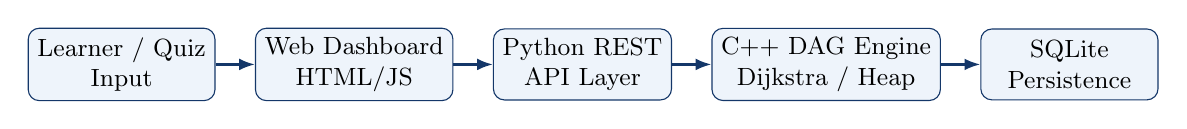
\begin{tikzpicture}[node distance=5mm,
box/.style={rectangle,rounded corners,draw=GEUBlue,fill=GEULightBlue,minimum width=2.25cm,minimum height=9mm,align=center,font=\small},
arrow/.style={-{Latex[length=2mm]},thick,draw=GEUBlue}]
\node[box](a){Learner / Quiz\\Input};
\node[box,right=of a](b){Web Dashboard\\HTML/JS};
\node[box,right=of b](c){Python REST\\API Layer};
\node[box,right=of c](d){C++ DAG Engine\\Dijkstra / Heap};
\node[box,right=of d](e){SQLite\\Persistence};
\draw[arrow](a)--(b);
\draw[arrow](b)--(c);
\draw[arrow](c)--(d);
\draw[arrow](d)--(e);
\end{tikzpicture}
\vspace{3mm}
\begin{columns}[T,totalwidth=\textwidth]
\column{.48\textwidth}
\textbf{Major Components}
\begin{itemize}\itemsep2pt
\item C++ graph, heap, path finders
\item Python backend and REST endpoints
\item SQLite relational data and audit logs
\item Web SPA: Vis.js and Chart.js
\end{itemize}
\column{.48\textwidth}
\textbf{System Flow}
\begin{itemize}\itemsep2pt
\item Learner input / quiz submission
\item Proficiency and effective weights updated
\item Path optimizer recalculates route
\item Dashboard displays trajectory and metrics
\end{itemize}
\end{columns}
\end{frame}

% SLIDE 7: TECH STACK
\begin{frame}{Final Technology Stack}
\begin{columns}[T,totalwidth=\textwidth]
\column{.48\textwidth}
\begin{block}{Software / Technologies}
\begin{itemize}\itemsep2pt
\item Programming: C++17, Python 3.12
\item Database: SQLite3
\item Frontend: HTML5, CSS, JavaScript ES6
\item Visualization: Vis.js, Chart.js
\item API payloads: JSON
\end{itemize}
\end{block}
\column{.48\textwidth}
\begin{block}{Development Infrastructure}
\begin{itemize}\itemsep2pt
\item Build: Make / CMake support
\item Version Control: Git, GitHub
\item Testing: C++ unit tests, Python API tests
\item Server: Python HTTP server / REST API
\item Concurrency: std::thread, worker pools, mutexes
\end{itemize}
\end{block}
\end{columns}
\end{frame}

% SLIDE 8: COURSE CONCEPTS
% SLIDE 8: COURSE CONCEPTS
\begin{frame}{Implementation of PBL Course Concepts}
\scriptsize
\begin{center}
\renewcommand{\arraystretch}{1.25}
\begin{tabularx}{.96\textwidth}{@{}>{\bfseries\RaggedRight}p{2.3cm} >{\RaggedRight\arraybackslash}X >{\RaggedRight}p{2.6cm}@{}}
\toprule
Course & Concepts Implemented & Project Module\\
\midrule
Data Structures & Directed graphs, adjacency/predecessor lists, custom binary min-heap, Dijkstra, topological sorting & Curriculum DAG and route planner\\
OOP with C++ & Abstract interfaces, polymorphism, encapsulation, RAII, smart pointers & IPathFinder and path-finder implementations\\
Operating Systems & Threads, worker pools, mutex synchronization, concurrency simulation & OSConcurrencySimulator\\
DBMS & Relational schema, six tables, foreign keys, indexes, ACID transactions, audit logging & SQLite persistence and transaction logger\\
\bottomrule
\end{tabularx}
\end{center}
\vfill
\begin{center}
\colorbox{GEULightBlue}{\parbox{.9\textwidth}{\centering\textbf{Course concepts are tied to implemented modules and reported validation evidence.}}}
\end{center}
\end{frame}

% SLIDE 9: MODULES
\begin{frame}{Module-Wise Final Implementation}
\scriptsize
\begin{center}
\renewcommand{\arraystretch}{1.3}
\begin{tabularx}{.96\textwidth}{@{}p{2.5cm}X p{2.2cm}p{1.4cm}@{}}
\toprule
\textbf{Module} & \textbf{Implementation} & \textbf{Responsible} & \textbf{Status}\\
\midrule
REST API / Backend & Python 3.12 server and backend service with 12 endpoints & Priyanshi Saini & Complete\\
Database / ACID Audit & SQLite schema, normalized tables, constraints, transaction logger & Ishita Doval & Complete\\
OS Simulation / Tests & Worker threads, mutexes, C++ unit tests and Python API test suite & Navdeep Singh Pundir & Complete\\
Dashboard & SPA, live DAG visualization, topic inspectors and benchmark charts & Team & Complete\\
Adaptive Weight Engine & Proficiency-based weight calculation, deficit penalties, rerouting & Priyanshi and Ishita & Complete\\
Benchmark & Static/adaptive comparisons across 8 milestone goals & Navdeep and Team & Complete\\
\bottomrule
\end{tabularx}
\end{center}
\vspace{3mm}
\begin{center}\colorbox{GEULightBlue}{\parbox{.7\textwidth}{\centering\textbf{Reported Phase-III milestone completion: 100\%}}}\end{center}
\end{frame}

% SLIDE 10: DEMO
\begin{frame}{Working System / Prototype Demonstration}
\begin{columns}[T,totalwidth=\textwidth]
\column{.43\textwidth}
\textbf{Major Working Features}
\begin{itemize}\itemsep3pt
\item Learner authentication / session handling
\item Knowledge DAG visualization
\item Quiz and proficiency updates
\item Adaptive path calculation and rerouting
\item Dashboard analytics and benchmark telemetry
\end{itemize}
\column{.53\textwidth}
\begin{block}{System Screenshot / Output}
\centering\vspace{10mm}
\placeholder{Add screenshot of the live dashboard here.}\\
\vspace{10mm}
\end{block}
\end{columns}
\smallnote{Use a live demonstration when possible; screenshots should support the demonstration.}
\end{frame}

% SLIDE 11: BACKEND AND DATABASE
\begin{frame}{Data / Database / Backend Implementation}
\begin{columns}[T,totalwidth=\textwidth]
\column{.48\textwidth}
\textbf{Database / Data}
\begin{itemize}\itemsep3pt
\item SQLite database: pbl\_curriculum.db
\item Six normalized tables
\item Students, topics, prerequisites, proficiency, quiz questions, learning paths
\item Foreign-key constraints and B-tree indexes
\item ACID transaction audit logging
\end{itemize}
\column{.48\textwidth}
\textbf{Backend / Core Logic}
\begin{itemize}\itemsep3pt
\item Python 3.12 server and backend service
\item 12 REST API endpoints
\item JSON request/response schema
\item Quiz assessment and proficiency update
\item Adaptive path recalculation and rerouting
\end{itemize}
\end{columns}
\end{frame}

% SLIDE 12: TESTING
\begin{frame}{Testing \& Validation}
\scriptsize
\begin{center}
\renewcommand{\arraystretch}{1.25}
\begin{tabularx}{.96\textwidth}{@{}p{2.4cm}p{1.5cm}X@{}}
\toprule
\textbf{Test Type} & \textbf{Status} & \textbf{Validation Scope / Result}\\
\midrule
Min-Heap and Dijkstra & Pass & Shortest-path correctness on 15-node knowledge DAG\\
Kahn topological sort / cycles & Pass & Valid prerequisite ordering; rejects circular edges\\
Dynamic weight and reroute & Pass & Weights follow formula and route adapts to prerequisite deficit\\
Multithreaded OS simulation & Pass & 100 concurrent learners in reported 13.8 ms; 7,264 ops/sec\\
Database constraints / transactions & Pass & Foreign-key cascades, unique constraints, ACID audit logging\\
REST API endpoints & Pass & Reported 100\% pass rate; average latency below 15 ms\\
\bottomrule
\end{tabularx}
\end{center}
\begin{block}{Validation Summary}
Phase-III report records passing C++ and Python test suites, database validation, adaptive rerouting tests, and concurrency simulation. Larger real-world stress testing can be presented as future validation if further evidence is collected.
\end{block}
\end{frame}


% SLIDE 13: RESULTS
\begin{frame}{Results \& Performance Analysis}
\begin{columns}[T,totalwidth=\textwidth]
\column{.48\textwidth}
\textbf{Reported Key Results}
\begin{itemize}\itemsep3pt
\item 35.1\% average study-time reduction
\item 18.9 hours average saved
\item 88.5\% projected concept retention
\item API average latency below 15 ms
\item 7,264 concurrency operations/sec
\end{itemize}
\column{.48\textwidth}
\begin{block}{Benchmark Summary}
\centering
\begin{tabular}{@{}lr@{}}
Static average & 53.8 h\\
Adaptive average & 34.9 h\\
Time saved & 18.9 h\\
Reduction & 35.1\%\\
\end{tabular}
\vspace{2mm}
\small Reported across eight milestone goals.
\end{block}
\end{columns}
\end{frame}

% SLIDE 14: REPO
\begin{frame}{GitHub Repository \& Development Evidence}
\begin{columns}[T,totalwidth=\textwidth]
\column{.45\textwidth}
\textbf{Repository Details}
\begin{itemize}\itemsep3pt
\item Repository: \href{https://github.com/sainipriyanshi842-collab/personalized-learning-and-path-optimisation}{GitHub Project Repository}
\item Branch: main
\item Stack: C++17, Python 3.12, SQLite3, HTML/CSS/JS
\item Source, database, web, and tests directories
\end{itemize}
\column{.51\textwidth}
\textbf{Development Evidence}
\begin{itemize}\itemsep3pt
\item C++ DAG and min-heap source
\item Python REST backend files
\item SQL schema and transaction scripts
\item Frontend dashboard source
\item Unit tests, API tests, benchmark outputs
\end{itemize}
\end{columns}
\vfill
\begin{center}\colorbox{GEULightBlue}{\parbox{.88\textwidth}{\centering\textbf{Repository:} \\ \url{https://github.com/sainipriyanshi842-collab/personalized-learning-and-path-optimisation}}}\end{center}
\end{frame}

% SLIDE 15: INDIVIDUAL CONTRIBUTIONS
\begin{frame}{Individual Contribution}
\scriptsize
\begin{center}
\renewcommand{\arraystretch}{1.35}
\begin{tabularx}{.96\textwidth}{@{}p{2.1cm}p{2.3cm}X@{}}
\toprule
\textbf{Member} & \textbf{Role} & \textbf{Technical Contribution}\\
\midrule
Priyanshi Saini & Team Lead / Backend & REST API architecture, Python server, endpoints, dashboard coordination, optimizer integration\\
Ishita Doval & Database Lead & SQLite schema, normalized tables, indexes, constraints, transaction and audit logging\\
Navdeep Singh Pundir & Testing Lead & OS concurrency simulator, thread synchronization, C++ unit tests, Python API tests, benchmark verification\\
\bottomrule
\end{tabularx}
\end{center}
\end{frame}

% SLIDE 16: DYNAMIC WEIGHT FORMULA
% SLIDE 16: DYNAMIC WEIGHT FORMULA
\begin{frame}{Adaptive Weight Optimization}
\footnotesize
\setlength{\abovedisplayskip}{3pt}
\setlength{\belowdisplayskip}{3pt}
For each topic \(v\), the dynamic effective study weight is calculated from baseline hours, proficiency, and prerequisite deficit:
\[
W'(v)=W(v)\left[1+\alpha\left(1-P(v)\right)\right]+\operatorname{PrereqPenalty}(v), \qquad
\operatorname{PrereqPenalty}(v)=\sum_{\substack{u\in\operatorname{Pred}(v)\\P(u)<0.60}}1.5\left(0.60-P(u)\right)
\]
\begin{itemize}\itemsep1pt\parskip0pt
\item \(W(v)\): baseline topic hours; \(P(v)\): assessed proficiency (\(0\text{--}1\)); \(\alpha=0.35\) sensitivity coefficient.
\item Mastery fast-track review floor is reported as \(0.15\times W(v)\).
\end{itemize}
\vspace{-1mm}
\begin{block}{Example: Topic T05 (Recursion \& Backtracking, baseline 6 h)}
\begin{itemize}\itemsep1pt\parskip0pt
\item Unattempted (\(P=0\)): \(8.10\text{ h}\) effective weight.
\item Mastered (\(P=0.90\)): \(6.21\text{ h}\) formula result; fast-track review floor \(0.90\text{ h}\).
\item Prerequisite T04 proficiency \(0.20\) adds \(0.60\text{ h}\) penalty, yielding \(8.70\text{ h}\).
\end{itemize}
\end{block}
\end{frame}

% SLIDE 17: BENCHMARK DETAILS
\begin{frame}{Static vs Adaptive Benchmark Results}
\scriptsize
\begin{center}
\renewcommand{\arraystretch}{1.15}
\begin{tabularx}{.97\textwidth}{@{}cXrrr@{}}
\toprule
Goal & Topic & Static (h) & Adaptive (h) & Saved (h)\\
\midrule
T04 & Stacks \& Queues & 16.0 & 1.7 & 14.3\\
T06 & Binary Trees \& Traversals & 27.5 & 18.9 & 8.6\\
T07 & BST \& Balanced Trees & 34.0 & 28.6 & 5.4\\
T10 & Graph Traversals (BFS/DFS) & 48.5 & 25.9 & 22.6\\
T12 & Dijkstra's Shortest Path & 60.5 & 45.4 & 15.1\\
T13 & Minimum Spanning Trees & 67.0 & 44.8 & 22.2\\
T14 & Dynamic Programming & 75.0 & 31.5 & 43.5\\
T15 & Graph Dynamic Programming & 82.5 & 70.0 & 12.5\\
\midrule
Overall & Full Curriculum Average & 53.8 & 34.9 & 18.9\\
\bottomrule
\end{tabularx}
\end{center}
\vspace{2mm}
\begin{center}\colorbox{GEULightBlue}{\parbox{.8\textwidth}{\centering\textbf{Reported overall study time reduction: 35.1\%}}}\end{center}
\end{frame}

% SLIDE 18: CONCLUSION
\begin{frame}{Conclusion \& Future Work}
\begin{block}{Conclusion}
Phase-III reports a full-stack adaptive learning system combining graph algorithms, learner assessment, persistent database transactions, REST services, interactive visualization, and concurrency testing. The system aims to generate prerequisite-valid personalized learning paths and reduce unnecessary study effort.
\end{block}
\textbf{Future Work / Further Validation}
\begin{itemize}\itemsep3pt
\item Expand stress tests with larger learner cohorts and longer workloads.
\item Collect more empirical learner feedback and retention measurements.
\item Extend analytics and personalize scheduling using additional learner preferences.
\item Improve deployment, documentation, and usability testing.
\end{itemize}
\end{frame}

% SLIDE 19: THANK YOU
\begin{frame}[plain]
\begin{tikzpicture}[remember picture,overlay]
\draw[GEUBlue,line width=3pt](current page.north west)--(current page.north east);
\node[align=center,text width=.8\paperwidth] at (current page.center){
{\color{GEUBlue}\fontsize{30}{36}\selectfont\bfseries THANK YOU}\\[4mm]
{\Large Questions and Discussion}\\[5mm]
{\large Personalized Learning Path Optimization}\\
{\normalsize Team Rockets | DSCPP-III-2026-T284}};
\node[align=center,anchor=south,yshift=.45cm] at (current page.south){\small Department of Computer Science \& Engineering\\Graphic Era (Deemed to be University), Dehradun};
\end{tikzpicture}
\end{frame}

\end{document}
